\begin{figure*}[hb]
    \centering 
    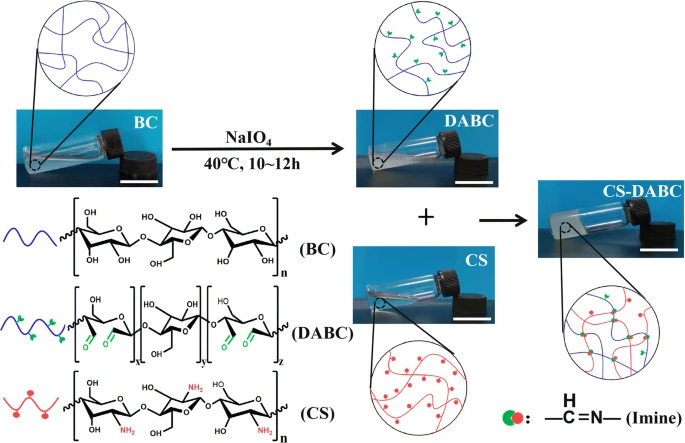
\includegraphics[width=0.7\linewidth]{Figures/CS_DABC_condensation.jpg}
    \caption{Schematic representation of hydrogel synthesis from chitosan and dialdehyde bacterial cellulose \autocite{liAllnaturalInjectableHydrogel2020}}
    \label{fig:CS_DABC_condensation}
\end{figure*}

\section{Towards a Self-Healing JTA}

A recent study by \citeauthor{liAllnaturalInjectableHydrogel2020} found that an all-natural, injectable hydrogel could be synthesized using chitosan and dialdehyde bacterial cellulose (\citeyear{liAllnaturalInjectableHydrogel2020}). This hydrogel uses imine bond dynamic cross-linkages to achieve its self-healing properties, where the Schiff base forms through the reaction of chitosan (as the amine) and bacterial cellulose (as the aldehyde).
The reaction can proceed under mild conditions (room temperature and pH = 7.2), and as it is all-natural, it has shown to be biocompatible. A schematic representation of this condensation reaction is given in Figure~\ref{fig:CS_DABC_condensation}.

Researchers tested the CS-DABC hydrogel's ability to self-repair after sustaining damage, a property that is desired for applications in wound dressings. To do so, round hydrogels were prepared and cut in half. One side was coloured orange, and the two half-discs were placed side-by-side in ambient conditions, as shown in Figure~\ref{fig:CS_DABC_self_healing}.
In just 3 hours, without external intervention, the two halves fused back together and reformed the original shape. They were also able to be picked up by one side, withstanding the force of gravity. Moreover, the gaps between the two hydrogel half-discs were observed under optical microscope.
The boundaries between the two sides were barely visible, demonstrating good self-healing properties from Schiff base reactions.

\begin{figure}[ht]
    \centering 
    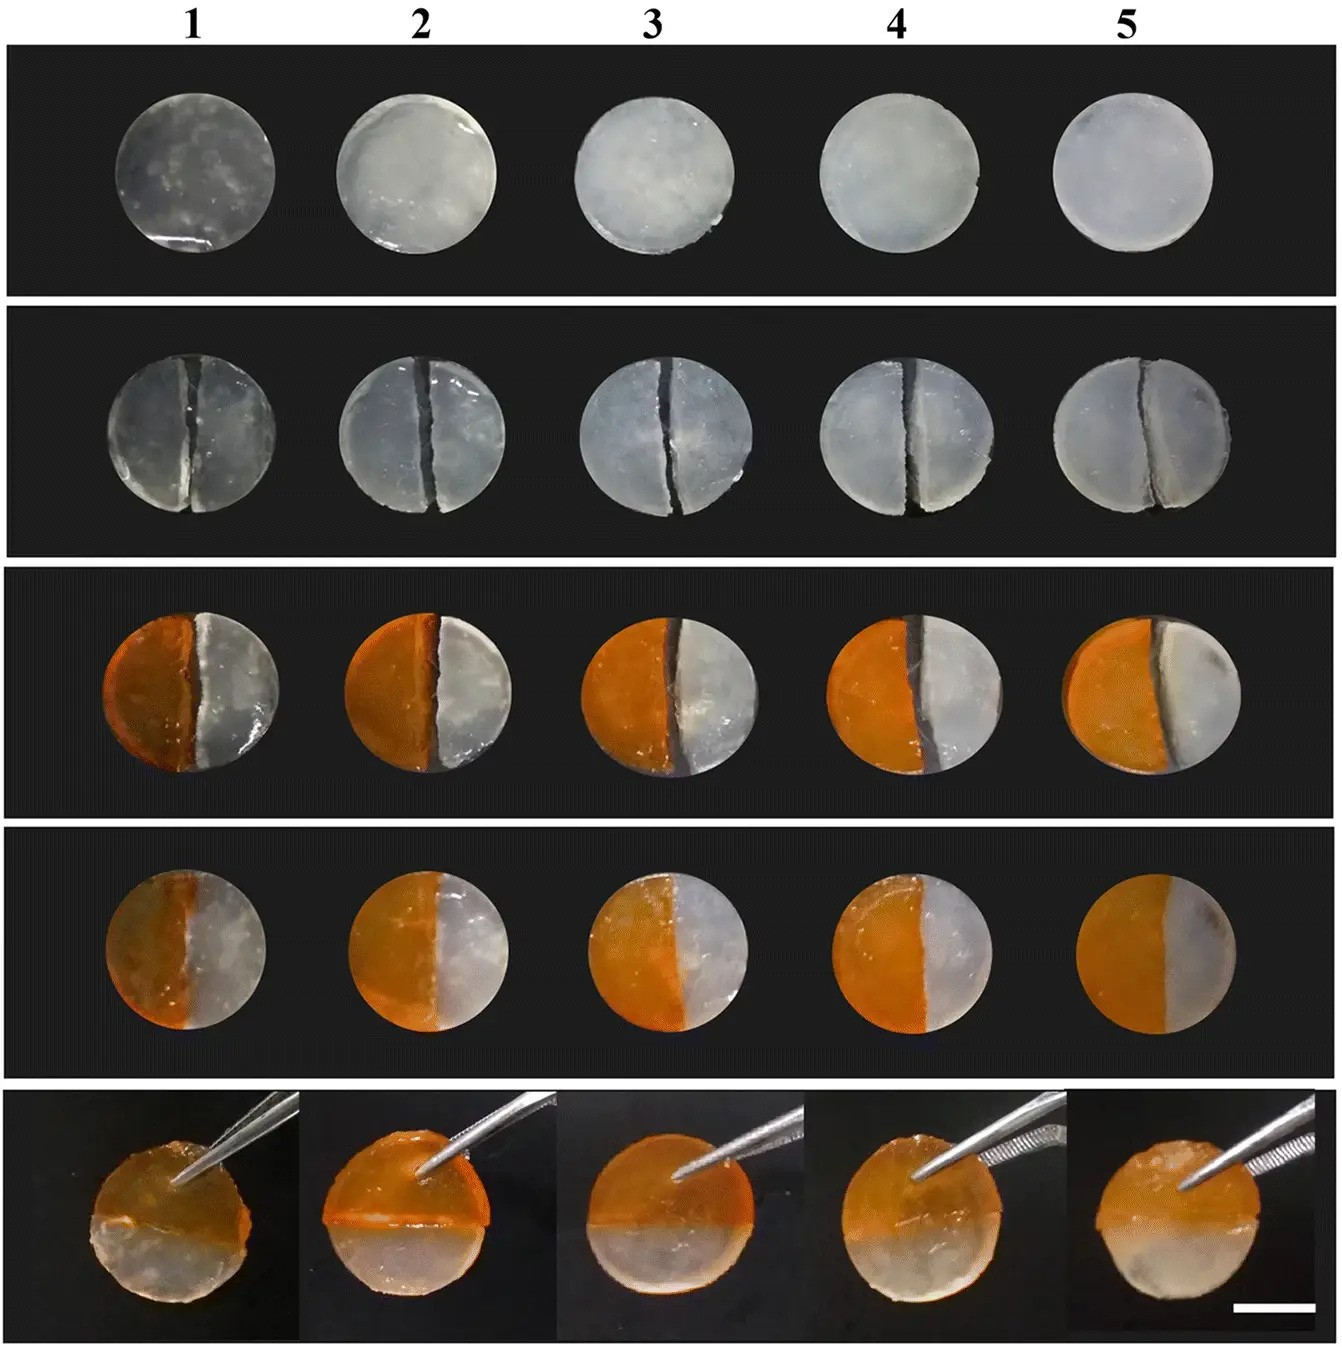
\includegraphics[width=\linewidth]{Figures/CS_DABC_self_healing.jpg}
    \caption{Self-healing properties of CS-DABC hydrogels. Discs were cut, stained, and healed under ambient conditions. [Adapted from \cite{liAllnaturalInjectableHydrogel2020}]}
    \label{fig:CS_DABC_self_healing}
\end{figure}

Additionally, the chitosan dressing exhibits antimicrobial properties, which reduces the risk of cross-contamination and promotes healthy healing of the wound. To evaluate these properties, the hydrogel was tested as an antibiotic against strains of \textit{E. coli} and \textit{S. aureus}.
Far fewer bacterial colonies were observed in the samples treated with CS-DABC compared to the control. As the hydrogel's protonated amino groups bind to the bacterial cell wall, effectively destroying it, bacterial growth is inhibited \autocite{liAllnaturalInjectableHydrogel2020}.

This self-healing hydrogel presents a promising application for tendon repair. Since JTAs already have a chitosan layer, it could be possible to synthesize Schiff bases directly on the existing structure using a similar technique as \citeauthor{liAllnaturalInjectableHydrogel2020}, leading to increased mechanical strength through the integration of self-healing properties.
% This self-healing hydrogel, therefore, has an interesting application for tendon repair. Given that JTAs have a chitosan side, it could be possible to augment their mechanical strength by integrating self-healing properties.